\chapter[Metodologia]{Metodologia}

Foi desenvoldido uma ferramenta para geração de forma automática de mapas aleatórios ou com uma repetição de padrão. Pode ser definido um percurso minimo para evitar seja gerados mapas onde o ponto inicial e final estão muito próximos.
Os mapas gerados para analise são de tamanho 100x100, com um padrão de repetição de 5x5 que é gerado de forma aleatória, para todos os mapas o percurso minimo de 15 passos.

No total foram gerados 800 mapas, sendo dividos em 400 aleatórios e 400 com repetição de padrão.
Os 400 mapas de cada são divididos em 100 para cada tipo de diagonal, isso deve pelo motivo que dependendo do tipo movimentação diagonal do mapa, ele pode ou nar ter uma solução.

As movimentações diagonais possiveis são:

\textbf{Nunca}: não permite andar nas verticais, podendo somente se movimentar para cima, baixo, direita e esquerda.

\textbf{Sempre}: permite ir para qual direção.

\begin{minipage}{\linewidth}
    \makebox[\linewidth][c]{
        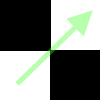
\includegraphics[keepaspectratio=true,scale=1]{ibagens/d_aways.png}}
    \captionof{figure}{Movimentação diagonal Sempre}
    \label{fig:d_aways}
\end{minipage}

\textbf{No máximo um obstaculo}: é permitidos seguir na vertical, se um dos lados estiver livre.

\begin{minipage}{\linewidth}
    \makebox[\linewidth][c]{
        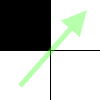
\includegraphics[keepaspectratio=true,scale=1]{ibagens/d_one.png}}
    \captionof{figure}{Movimentação diagonal Apenas um obstaculo}
    \label{fig:d_one}
\end{minipage}


\textbf{Apenas sem obstáculos}: é permitidos seguir na vertical, se os dois dos lados estiver livre.

\begin{minipage}{\linewidth}
    \makebox[\linewidth][c]{
        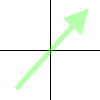
\includegraphics[keepaspectratio=true,scale=1]{ibagens/d_noobstacle.png}}
    \captionof{figure}{Movimentação diagonal Sem obstaculo}
    \label{fig:d_noobstacle}
\end{minipage}


Os algoritmos de busca utilizados para os teste são A\**, BFS, Dijkstra e IDA\**, sendo executados uma vez para cada uma das heurística selecionadas para os testes, essas são Manhattam, Euclideana, Octil e Chebyshev.

Para o GA cada resultado de cada configuração é gerado 10 vezes, depois é realizado uma média dessas tentativas para comparação posterior com os algoritimos classicos. As possíveis configurações são definidas por todos operadores de cruzamento, mutação, seleção, aptidão e heurísticas.Os operados de cruzamento são simples, OBX e o PBX. Os operadores de Mutação são Bitwise, DIVM, DM, EM, IM,IVM e SM. Na seleção utilizamos o algoritmo de Roleta. A função de aptidão é uma função baseada nas heurísticas implementadas, uma sem nenhuma alteração, outra penalizando caminhos cíclicos, outra penalizando encontro com paredes e mais uma penalizando tanto caminhos cíclicos quanto encontro com paredes.

Os dados coletados são acumulados de duas formas, uma forma consolidada que mistura os algoritmo de busca com os dados do GA para comparação, e uma forma especifica para o GA, para analisar as configurações do GA para as diferentes situações.

\chapter[Implementação]{Implementação}

Nesse capitulo será apresentado mais aprofundadamente as ferramentas e métodos que foram utilizados para realizar os testes  e implemetações dos modelos de busca de caminho.

\section{Tecnologias}
O projeto é separado em Pathfinder e Pathfinder.UI ambos desenvolvidos na linguagem C\# o primeiro utilizando o .NET Standard Library 1.6 e o segundo no .NET Core. No projeto Pathfinder estão todas a  implementações dos algoritmos de busca que temos para a comparação. Pathfinder.UI tem como objetivo consumir os recusursos do projeto Pathfinder, dando opções de visualização ou geração de dados. Ambos rodam em sistemas Windows e \**nix utilizando o .Net Core CLI 1.1 para execução.

\section{Estrutura do Projeto}

Essa seção tem como objetivo descrever como foram implementados os algoritmos 

\subsection {PathFinder}

Projeto de implementação de algoritmos de busca.
Sua estrutura de pastas está organizada em Abstraction, Core, Factories, Finders, GeneticAlgorithm, Heuristics e MapGenerators.

O \textbf{'project.csproj'} é o arquivo onde é definido as bibliotecas utilizadas e a versão do .NET Framework, as outras pastas agregam arquivos com informações relevantes a nossa implementação.

\subsection{Abstraction}	

Nesta pasta estão todos os arquivos a nível de abstração dos algoritmos de busca, esses são:

\textbf{IFactory}: Essa interface tem como objetivo padronizar as "fabricas", ferramentas que decidir e instanciar toda dependência necessária.

\textbf{IMap}: Essa interface tem como objetivo abstrair o comportamento da classe de mapa utilizada nos arquivos de busca, assim sendo por padrão todo algoritmo espera uma implementação de IMap para rodar.

\textbf{IHeuristic}: Essa interface abstrai o comportamento das heurísticas.

\textbf{IMapGenerator}: Essa interface tem como objeto abstrair os gerador de mapas.

\textbf{IFinder}: Essa interface é a responsável por abstrair todo comportamento dos algoritmos de busca.

\textbf{IGeneticAlgorithm}: Essa interface herda de IFinder, ela compartilha a mesma assinatura de métodos, propriedades e eventos, porem acrescenta a abstração necessária para
o utilização de GA.


\subsection{Core}

Nesta pasta são definidos as implementações e configurações bases.

\textbf{Container}: Esta classe é responsável por registar e resolver as implementações conhecidas das interfaces.

\textbf{Enumerators}: Contem as definições de enumerações, usados para usar nomes bem definidos ao invés de números avulsos no código.

\textbf{Extensions}: Arquivo com métodos auxiliares de lista para comportamento de uma estrutura de pilha.

\textbf{FileTools}: Classe responsável por toda manipulação de I/O de arquivos

\textbf{Map}: Implementação do IMap, tem como objetivo ser a estrutura de mapa base dos algoritmos de busca.

\textbf{Node}: Classe responsável por ser a representação de uma célula no mapa, ou seja, o mapa é uma matriz de \textbf{\textit{"Node"}}.

\textbf{Settings}: Contém toda configuração estática do projeto, do qual é carregado de um arquivo Json chamado "appsettings.json"

\subsection{Factories}

Nesta Pasta temos os arquivos responsáveis pelo instanciar as implementações de interfaces.

\textbf{FinderFactory}: Classe responsável por decidir e instanciar uma implementação IFinder.

\textbf{HeuristicFactory}: Classe responsável por decidir e instanciar uma implementação IHeuristic.

\textbf{MapGeneratorFactory}: Classe responsável por decidir e instanciar uma implementação IMapGenerator.

\subsection{Finders}

Nesta pasta temos definidas as implementações de todos os algoritmos de busca de caminho.

\textbf{AStarFinder}: Implementação do algoritmo de busca de caminho A* implementada em cima da interface IFinder.

\textbf{BestFirstSearchFinder}: Implementação do algoritmo de busca de caminho “Best First Search” implementada em cima da interface IFinder.

\textbf{DijkstraFinder}: Implementação do algoritmo de busca de caminho Dijkstra implementada em cima da interface IFinder.

\textbf{IDAStarFinder}: Implementação do algoritmo de busca de caminho IDA* implementada em cima da interface IFinder.

\textbf{GAFinder}: Implementação de um algoritmo genético para busca de caminhos implementada em cima da interface IFinder e IGeneticAlgorithm.

\subsection{Heuristics}

Nesta pasta são definidas as implementações de IHeuristic, responsáveis pelos cálculos de heurística.

\textbf{Manhattan}: Implementação da classe Manhattan implementada em cima da interface IHeuristic responsável por calcular a distancia Manhattam.

\textbf{Euclidean}: Implementação da classe Euclidean implementada em cima da interface IHeuristic responsável por calcular a distancia Euclideana.

\textbf{Octile}: Implementação da classe Octile implementada em cima da interface IHeuristic responsável por calcular a distancia Octile.

\textbf{Chebyshev}: Implementação da classe Chebyshev implementada em cima da interface IHeuristic responsável por calcular a distancia Chebyshev.

\section{Genetic Algorithm}

Nesta pasta são definidos todas as implementações referentes ao algoritmo genético, pela complexidade.
do algoritmo ele possui uma estrutura própria de pastas para definições e configurações de injeção de dependência.

\subsection{Abstraction}

Nesta pasta estão todos os arquivos a nível de abstração das etapas do algoritmo genético.

\textbf{ISelection}: Interface é responsável por abstrair os algoritmos de seleção.

\textbf{IGenome}: Interface tem como funcionalidade abstrair a definição de genoma.

\textbf{IFitness}: Interface tem como objetivo abstrair o calculo de fitness.

\textbf{IMutate}: Interface tem como objetivo abstrair os operadores de mutação.

\textbf{ICrossover}:  Interface tem como objetivo abstrair os operadores de cruzamento.

\textbf{IRandom}: Interface tem como objetivo abstrair a implementação de geração de números aleatórios.

\textbf{AbstractMutate}: Implementação base para operador de mutação.

\textbf{AbstractCrossover}: Implementação base para operador de cruzamento.

\subsection{Core}

\textbf{Adaptation}: Classe responsável para realizar a adaptação de um indivíduo novo após ser gerado.

\textbf{Enumerators}: Contem as definições de enumerações, usados para usar nomes bem definidos ao invés de números avulsos no código.

\textbf{GARandom}: Implementação responsável por gerar números aleatórios, implementa IRandom.

\textbf{GASettings}: Arquivo responsável por carregar configuração estática de GA, carrega do arquivo "GASettings.json”.

\textbf{Genome}: Classe responsável por representar o genoma no algoritmo de GA, implementa a IGenome.


\subsection{Selection}

Nesta pasta estão todas as implementações dos algoritmos de seleção.

\textbf{SelectionRandom}: Implementação de seleção de indivíduos aleatório.
\textbf{SelectionRouletteWheel}: Implementação de seleção roleta.

\subsection{Crossover}

Nesta pasta estão todas as implementações dos algoritmos de cruzamento.

\textbf{CrossoverOBX}: Implementação do operador de cruzamento OBX.

\textbf{CrossoverPBX}: Implementação do operador de cruzamento PBX.

\textbf{CrossoverSimple}:  Implementação do operador de cruzamento simples.

\subsection{Mutation}

Nesta pasta estão todas as implementações dos algoritmos de mutação.

\textbf{MutateBitwise}: Implementação do operador de cruzamento Bitwise.

\textbf{MutateDIVM}: Implementação do operador de cruzamento DIVM.

\textbf{MutateDM}: Implementação do operador de cruzamento DM.

\textbf{MutateEM}: Implementação do operador de cruzamento EM.

\textbf{MutateIM}: Implementação do operador de cruzamento IM.

\textbf{MutateIVM}: Implementação do operador de cruzamento IVM.

\textbf{MutateSM}: Implementação do operador de cruzamento SM.


\section{Projeto de UI}

Foi desenvolvido um projeto com objetivo de consumir a biblioteca de busca de caminhos, e poder visualiza-los.

\subsection{Abstraction}

Nesta pasta estão todos os arquivos a nível de abstração.

\textbf{IAppMode}: Abstração que define de que forma o app ira rodar.

\textbf{IViewer}: Abstração do tipo de visualizador.

\subsection{AppMode}

Pode-se configurar diferentes modos de rodar os algoritmo, nesse pasta estão a implementação das diferentes formas.

\textbf{SingleRunMode}: O programa será executado e rodara uma vez usando as configurações do arquivo estático "appsettings.json" que é lido pela classe UISettings.

\textbf{DynamicMode}: O programa ira perguntar qual algoritmo, heurística, tipo de diagonal, forma de visualização e cada operador do GA antes de rodar.

\textbf{BatchMode}: O software ira rodar N vezes cada algoritmo selecionado no arquivo de configuração, onde N também é definido neste arquivo, ao final ira salvar os resultados e cada mapa numa pasta na raiz do projeto.


\subsection{Core}

Nesta pasta são definidos as implementações e configurações bases.

\textbf{Enumerators}: Contem as definições de enumerações, usados para usar nomes bem definidos ao invés de números avulsos no código.

\textbf{RegisterConfig}: Neste arquivo são configurados os binds do visualizador para injeção de dependência.

\textbf{Settings}: Onde são carregados as configurações estáticas do arquivo "appsettings.json", neste são configurações da forma de visualização e do Batch.

\subsection{Factories}

Nesta Pasta temos os arquivos responsáveis pelo instanciar as implementações de interfaces.

\textbf{AppModeFactory}: Classe responsável por decidir e instanciar uma Implementação de IAppMode.

\textbf{ViwerFactory}: Classe responsável por decidir e instanciar uma Implementação de IViewer.

\subsection{Viewer}

Nesta pasta estão as diferentes formas de exibir os resultados das buscas.

\textbf{ConsoleViewer}: Classe responsável por apresentar a busca de caminhos em ASC no Console da aplicação.

\textbf{OpenGLViewer}: Classe responsável por apresentar a busca em uma janela em OpenGL.

\textbf{OpenGLWindow}: Classe que é utilizada pela OpenGLViewer para mostrar a janela com uma grid que mostra o andamento dos algoritmos.

\section{Estrutura do GA}

A busca utilizando o GA, segue com as operações base de todo GA, que são seleção, cruzamento, adaptação e mutação. 
Para cada interação é gerada uma população, a função de aptidão é calculada para cada indivíduo da população, 
desses o indivíduo com o valor mais próximo de zero é selecionado como o melhor.

\subsection{Função de Aptidão}

Nesta pasta estão as implementações das funções fitness.

\textbf{FitnessHeuristic}: Para cada indivíduo da população é calculada uma aptidão com base em uma função heurística (Manhattam, Octile, Euclideana, Chebyshev)
previamente definida, o calculo é feito a partir do ponto final da lista do genoma do indivíduo até o ponto de destino do mapa
a soma de todos os resultados é a função de aptidão da população.

\textbf{FitnessWithCollisionDetection}: Para cada indivíduo da população é calculada a função de aptidão idêntica a FitnessHeuristic, porém no processo de adaptação adaptação os caminhos que aumentarem para um caminho inválido, que colidam ou saiam do mapa, são marcados,
posteriormente todos os indivíduos marcados são penalizados com a  soma de  um valor alto para diminuir o valor de sua aptidão na população.

\subsection{Adaptação}

Ela é importante para corrigir possíveis problemas nos indivíduos resultantes dos operadores de cruzamento ou mutação. Quando os cromossomos são reorganizados, 
o caminho novo que foi gerado pode levar para cima de um bloqueio ou para fora do mapa, então seguindo as direções indicadas no cromossomo, 
a posição no mapa é recalcula e só adiciona o cromossomo do indivíduo se for uma posição valida ou que não voltam para o mesmo lugar.
Para complementar o caminho do indivíduo, uma nova direção valida é adicionada e calculada, fazendo com que cada interação de adaptação, o caminho cresça.

\subsection{Mutação}

Todas as mutações executam se o indivíduo tiver mais do que 3 cromossomos e não afeta o primeiro cromossomo.
O primeiro cromossomo é a ligação com o ponto inicial e se for trocado de lugar, o caminho é quebrado. /cite{MatBuckland}

\section{Modo Batch}

O modo Batch do programa serve para poder gerar os dados necessários para a analise.

Para iniciar o processo do batch é necessario o mudar o \textit{AppMode} no arquivo "appsettings.json" para 2 e iniciar a aplicação Pathfinder.UI.


\subsection{Configuração}

A definição das configurações para o Batch ficam no arquivo "appsettings.json" onde são carregadas na classe UISettings posteriormente na aplicação. As chaves que interessam ao modo batch são:

\textbf{Width}: Tamanho em largura dos mapas.

\textbf{Height}: Tamanho em altura dos mapas.

\textbf{MinimumPath}: Tamanho minimo entre o ponto inicial e final dos mapas.

\textbf{RandomBlock}: Tamanho que sera usado para gerar aleatoriamente uma parte do mapa e se repetira para completar os mapas com padrão.

\textbf{Batch\_map\_origin}: Define se você quer carregar os mapas previamente gerados ou gerar mapas novos para a execução.

\textbf{Batch\_map\_qtd\_to\_generate}: Quantidade de mapas que serão gerados para o teste.

\textbf{Batch\_generate\_pattern}: Este campo define se os mapas gerados automaticamentes serão aleatorios (0) ou se terão algum padrão de repeticão (1).

\textbf{Batch\_map\_diagonal}: Define qual tipo de movimentação diagonal sera usada na geração dos mapas, onde Never(0), OnlyWhenNoObstacles(1), IfAtMostOneObstacle(2), Always(3).

\textbf{Batch\_GATimesToRunPerMap}: Define a quantidade de vezes que o GA ira rodar para cada configuração.

\textbf{Batch\_folder}: Pasta aonde serão gerados os mapas e arquivo de log do batch.

\textbf{Batch\_list\_finders}: Uma lista que define quais algoritimos de busca serão rodados no modo batch, as opçoes são  A\**(0), BFS(1), IDA\**(2), Dijkstra(3), GA(4).

\textbf{Batch\_list\_heuristics}: Uma lista que define quais heuristicas serão rodados no modo batch, as opçoes são Manhatam(0), Euclidean(1), Octile(2), Chebyshev(3).

\textbf{Batch\_list\_Mutation}: Uma lista que define quais operadores de mutação serão utilizados pelo GA no modo batch, as opçoes são  \textit{Exchange(0)}, \textit{Displaced Inversion}(1), \textit{Displacement}(2), \textit{Insertion}(3), \textit{Inversion}(4), \textit{Scramble}(5) e \textit{Bitwise}(6).

\textbf{Batch\_list\_Crossover}: Uma lista que define quais operadores de cruzamento serão utilizados pelo GA no modo batch, as opçoes são  \textit{Simple}(0), \textit{Order-Based Crossover}(1), \textit{Position-Based Crossover}(2).

\textbf{Batch\_list\_Fitness}: Uma lista que define quais funções de aptidão serão utilizados pelo GA no modo batch, as opçoes são Heuristica(0), Heuristica com penalidade em caminho ciclico(1), Heuristica com penalidade em caminhos que coliden(2) e Heuristica com penalidade em caminho ciclico e colisão(3).

\textbf{Batch\_list\_Selection}: Uma lista que define quais funções de seleção serão utilizados pelo GA no modo batch, as opçoes são  Aleatorio(0) e \textit{Roulette Wheel Selection}(1).

\section{Modo Visual}

O modo Visual do programa serve para poder rodar um algoritimo em um mapa especifico e acompanhar visualmente como ele se comporta.

Para iniciar o modo visual é necessario o mudar o \textit{AppMode} no arquivo "appsettings.json" para 0 e iniciar a aplicação Pathfinder.UI.


\subsection{Configuração}


A definição das configurações para o modo visual ficam no arquivo "appsettings.json" e "GASettings.json" onde são carregadas na classe UISettings posteriormente na aplicação. As chaves que interessam ao modo visual são:


\textbf{MapViwer}: Define o tipo de visualização que sera utilizada onde as opções são Console(0) e OpenGL(1).

\textbf{MapOrigin}: Define a origem do mapa utilizado no programa, onde as opções são Estatico(0), De um arquivo(1), Aleatorio(2), Com padrão(3).

\textbf{Heuristic}: Define qual heuristica sera rodado no modo visual, as opçoes são Manhatam(0), Euclidean(1), Octile(2), Chebyshev(3).

\textbf{AllowDiagonal}: Define qual tipo de movimentação diagonal sera usada, onde Never(0), OnlyWhenNoObstacles(1), IfAtMostOneObstacle(2), Always(3).

\textbf{Algorithm}: Define qual algoritmo de busca sera rodar no modo visual, as opçoes são  A\**(0), BFS(1), IDA\**(2), Dijkstra(3), GA(4).
 
\textbf{IDAStarFinderTimeOut}: Define em quanto tempo em milisegundos o IDA\** ira parar caso não encontre o caminho.

\textbf{IDATrackRecursion}: Define se ira mostrar todos os passos recursivos do IDA\** (pode demorar).
 
\textbf{RandomSeed}: Seed utilizada no gerador aleatorio de mapas.

\textbf{Width}: Tamanho em largura do mapa.

\textbf{Height}: Tamanho em altura do mapa.

\textbf{MinimumPath}: Tamanho minimo entre o ponto inicial e final do mapa.

\textbf{RandomBlock}: Tamanho que sera usado para gerar aleatoriamente uma parte do mapa e se repetira para completar o mapa com padrão.

\textbf{FileToLoad}: Arquivo de mapa que sera carregado caso escolhe o MapOrigin de arquivo.

\textbf{FolderToSaveMaps}: Pasta onde serão salvas altomaticamente os arquivos de mapas gerados.

\textbf{Start}: Define o caractere de ponto inicial no modo de visualização console.

\textbf{End}: Define o caractere de ponto final no modo de visualização console.

\textbf{Empty}: Define o caractere de caminho livre no modo de visualização console.

\textbf{Wall}: Define o caractere de parede no modo de visualização console.

\textbf{Path}: Define o caractere de caminho no modo de visualização console.

\textbf{Closed}: Define o caractere de nó fechado no modo de visualização console.

\textbf{Opened}: Define o caractere de nó aberto no modo de visualização console.

\textbf{OpenGlBlockSize}: Tamanho em pixel dos blocos no modo OpenGL.


\textbf{GenerationLimit}: Define o numero maximo de gerações do GA antes de abortar o processo.

\textbf{MutationRate}: Chance de ocorrer mutação em cada individuo de uma nova população.

\textbf{MutationAlgorithm}:  Define qual operador de mutação sera utilizados pelo GA no modo visual, as opçoes são  \textit{Exchange(0)}, \textit{Displaced Inversion}(1), \textit{Displacement}(2), \textit{Insertion}(3), \textit{Inversion}(4), \textit{Scramble}(5) e \textit{Bitwise}(6).

\textbf{CrossoverRate}: Chance de ocorrer cruzamento em cada par de individuos de uma nova população.

\textbf{CrossoverAlgorithm}: Define qual operador de cruzamento serão utilizados pelo GA no modo visual, as opçoes são  \textit{Simple}(0), \textit{Order-Based Crossover}(1), \textit{Position-Based Crossover}(2).

\textbf{PopulationSize}: Quantidade de individuos em cada nova população.

\textbf{FitnessAlgorithm}: Define qual função de aptidão sera utilizado pelo GA no modo visual, as opçoes são Heuristica(0), Heuristica com penalidade em caminho ciclico(1), Heuristica com penalidade em caminhos que coliden(2) e Heuristica com penalidade em caminho ciclico e colisão(3).

\textbf{SelectionAlgorithm}: Define qual função de seleção sera utilizado pelo GA no modo visual, as opçoes são  Aleatorio(0) e \textit{Roulette Wheel Selection}(1).

\textbf{BestSolutionToPick}: Quantidade de individuos mais bem avaliados a serem colocados em uma nova geração a partir da anterios.

\textbf{Penalty}: Valor de penalidade usado nas funções de aptdão.
